%%%%%%%%%%%%%%%%%%%%%%%%%%%%%%%%%%%%%%%%%%%%%%%%%%%%%%%%%%%%%%%%%%%%%%%%%%%%%%%%
%		      	             __   ____   ___  ____  __ _  ____ 
%                       / _\ (  _ \ / __)(  __)(  ( \(_  _)
%                 		 /    \ )   /( (_ \ ) _) /    /  )(  
%                      \_/\_/(__\_) \___/(____)\_)__) (__) 
%
% Argent Library
% Copyright (c) 2020 Abhishek Chakravarti <abhishek@taranjali.org>
%
% This file is part of the Argent Library. It provides the layout of the manual
% of the Argent Library.
%
% The contents of this file are released under the GPLv3 License. See the
% accompanying LICENSE file or the generated Developer Manual (section I:?) for 
% complete licensing details.
%
% BY CONTINUING TO USE AND/OR DISTRIBUTE THIS FILE, YOU ACKNOWLEDGE THAT YOU
% HAVE UNDERSTOOD THESE LICENSE TERMS AND ACCEPT TO BE LEGALLY BOUND BY THEM.
%%%%%%%%%%%%%%%%%%%%%%%%%%%%%%%%%%%%%%%%%%%%%%%%%%%%%%%%%%%%%%%%%%%%%%%%%%%%%%%%


\documentclass[a4paper, 10pt, twocolumn]{report}

\usepackage[english]{babel}
\usepackage{array}
\usepackage{booktabs}
\usepackage{fontawesome}
\usepackage{graphicx}
\usepackage{imakeidx}
\usepackage{fancyhdr}
\usepackage[backend=biber, bibencoding=utf8, minbibnames=5, maxbibnames=5,
    style=alphabetic, citestyle=authoryear]{biblatex}

\fancyhf{}
\fancyhead[LE]{\leftmark}
\fancyhead[RO]{\nouppercase{\rightmark}}
\fancyfoot[LE,RO]{\thepage}

\addbibresource{argent-manual.bib}
\makeindex[columns=3, title=Index, intoc]

\renewcommand{\familydefault}{\sfdefault}
\pagestyle{fancy}

\begin{document}

\begin{titlepage}
  \centering
  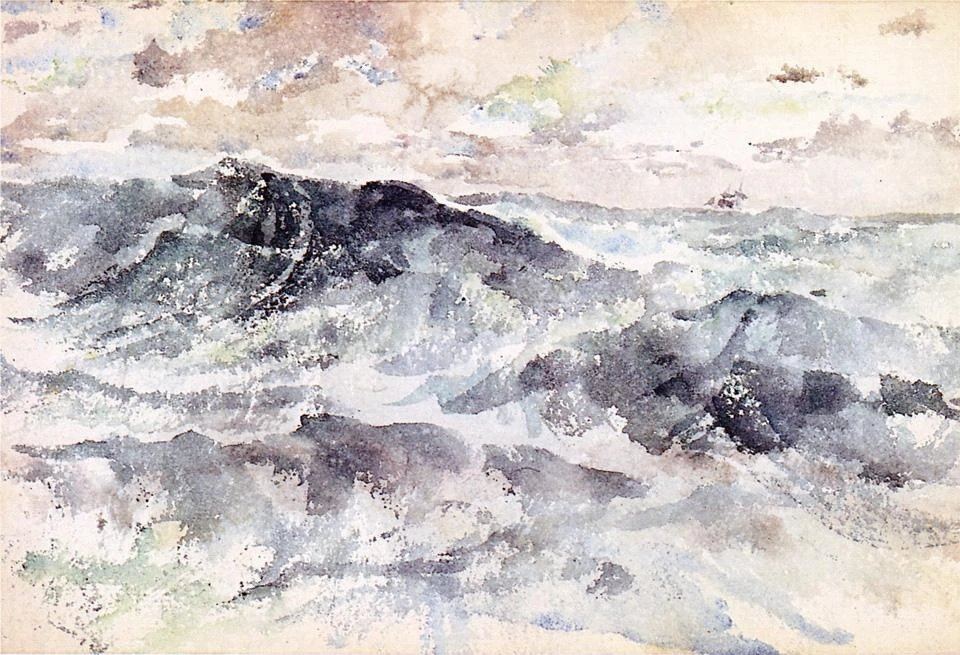
\includegraphics[width=0.95\textwidth]{the-great-sea.jpg}\par \vspace{1em}
  \Huge Argent Library \par \vspace{0.5em} \large v0.1.0 \par \vspace{0.5em} 
      \LARGE Developer Manual \par \vspace{5em} Abhishek Chakravarti \par
      \vspace{0.5em} \small abhishek@taranjali.org \vfill \large May 2020
\end{titlepage}

\tableofcontents
\listoffigures
\listoftables

\part{Overview}
\part{Application Programming Interface}
%https://www.overleaf.com/learn/latex/code_listing
\definecolor{GREEN}{rgb}{0,0.6,0}
\definecolor{GRAY}{rgb}{0.5,0.5,0.5}
\definecolor{PURPLE}{rgb}{0.58,0,0.82}
\definecolor{BACKGROUND}{rgb}{0.95,0.95,0.92}

\lstdefinestyle{CODE}{
  backgroundcolor=\color{BACKGROUND},
  commentstyle=\color{GREEN},
  keywordstyle=\color{blue},
  numberstyle=\tiny\color{GRAY},
  stringstyle=\color{PURPLE},
  basicstyle=\ttfamily\footnotesize,
  language=C,
  tabsize=4,
  showspaces=false,
  showstringspaces=false,
  frame=single,
  breaklines=true,
  captionpos=b,
  postbreak=\mbox{\textcolor{red}{$\hookrightarrow$}\space},
}
\lstset{style=CODE}


\chapter{Compiler Extensions}

\begin{bclogo}[logo=\bctrombone, noborder=true, couleurBarre=blue!30]{Files}
  \small
  \begin{tabular}{l l}
    \faPlug & \emph{src/api.h} \\
    \faWrench & \emph{src/api.h} \\
    \faBalanceScale & \emph{test/compiler-extensions.c} \\
    \faBook & \emph{doc/chapters/compiler-extensions.tex} \\
  \end{tabular}
\end{bclogo}

\begin{bclogo}[logo=\bctakecare, noborder=true, couleurBarre=orange]{Warning}
  The compiler extension macros have no effect on compilers other than GCC and
  Clang.
\end{bclogo}

GCC provides a rich set of compiler extensions to the C language standards
through the \verb|__attribute__| keyword. These compiler extensions allow 
special properties to be specified to types, enumerators, statements, functions, 
and variables. These special properties, applied through the 
\verb|__attribute__| keyword, are used by GCC to perform optimisations and
provide other enhancements beyond what the C standard specifies.

Experience has shown that careful use of these extensions is beneficial,
especially if we know that the code is to be compiled on GCC, or a GCC-
compatible compiler such as Clang that supports the \verb|__attribute__| 
keyword.

The Argent Library uses a few selected such extensions, and wraps them as macros
so that they degrade gracefully (with an appropriate warning) when ported to 
compilers that do not support the \verb|__attribute__| extensions provided
by GCC.

The list of compiler extension macros are summarised in Table~\ref{tab:synopsis}
and elaborated in the following sections. These macros are declared in the
\emph{src/api.h} header file.

\renewcommand\arraystretch{1.1}
\begin{table}[!htbp]
  \centering
  \small
  \begin{tabular}[t]{>{\centering}m{0.3\linewidth}
    >{\raggedright\arraybackslash}m{0.6\linewidth}}
    \toprule
    \textbf{Macro} & \textbf{Synopsis} \\
    \midrule
    \verb|ag_cold| & Hints that a given function is called rarely \\
    \verb|ag_hot| & Hints that a given function is called frequently \\
    \verb|ag_likely| & Hints that a predicate is likely to be true \\
    \verb|ag_pure| & Hints that a given function is pure \\
    \verb|ag_threadlocal| & Hints that a given variable has thread local 
      storage \\
    \verb|ag_unlikely| & Hints that a predicate is likely to be false \\
    \bottomrule
  \end{tabular}
  \caption{Synopsis of compiler extension macros}
  \label{tab:synopsis}
\end{table}


%%%%%%%%%%%%%%%%%%%%%%%%%%%%%%%%%%%%%%%%%%%%%%%%%%%%%%%%%%%%%%%%%%%%%%%%%%%%%%%%
% Macro ag_pure
%


\section{Macro \texttt{ag\_pure}}

  \begin{bclogo}[logo=\bccrayon, noborder=true, barre=snake, couleurBarre=gray]
    {Synopsis}
    \verb|#include <argent/api.h>|
    \verb|#define ag_pure| \ldots
  \end{bclogo}

  A \emph{pure function} is one that always returns the same result for the same
  set of arguments without any side effects. In order for GCC to consider a
  function to be pure, it must meet the following criteria:
  \begin{enumerate}
    \item Its return value depends only on its arguments and global variables.
    \item It does not modify any of its arguments or global variables.
    \item It does not involve any I/O calls such as \texttt{printf()}.
    \item It does not make a call to any impure function.
  \end{enumerate}

  By marking such functions as pure with the \texttt{ag\_pure} macro, GCC is able
  to perform relevant optimisations on them such as subexpression elimination. In
  order to mark a function as pure, apply the \texttt{ag\_pure} macro on the
  prototype declaration like so:

  \begin{lstlisting}[linewidth=1.0\linewidth, caption=Example use of ag\_pure]
    extern ag_pure int foo(const char *bar);
  \end{lstlisting}

  \begin{algorithmic}
    \If{$compiler = gcc$ or $compiler = clang$}
      \State{$\verb|ag_pure| \gets \verb|__attribute__((pure))|$}
    \Else
      \State{$\verb|ag_pure| \gets \emptyset$}\Comment{undefine ag\_pure}
      \State{\verb|#warning| $''message''$}
    \EndIf
  \end{algorithmic}


%%%%%%%%%%%%%%%%%%%%%%%%%%%%%%%%%%%%%%%%%%%%%%%%%%%%%%%%%%%%%%%%%%%%%%%%%%%%%%%%
% Macro ag_hot
%


\section{Macro \texttt{ag\_hot}}

\begin{bclogo}[logo=\bccrayon, noborder=true, barre=snake, couleurBarre=gray]
    {Synopsis}
  \verb|#include <argent/api.h>|
  \verb|#define ag_hot| \ldots
\end{bclogo}

A \emph{hot function} is one that is called frequently. Marking such hot
functions with the \verb|ag_hot| macro allows GCC to perform suitable
performance optimisations on them. To mark a function as hot, its prototype
needs to be decorated with \verb|ag_hot| like so:

\begin{lstlisting}[linewidth=1.0\linewidth, 
    caption=Example use of ag\_hot]
extern int foo(const char *bar) ag_hot;
\end{lstlisting}


%%%%%%%%%%%%%%%%%%%%%%%%%%%%%%%%%%%%%%%%%%%%%%%%%%%%%%%%%%%%%%%%%%%%%%%%%%%%%%%%
% Macro ag_cold
%


\section{Macro \texttt{ag\_cold}}

\begin{bclogo}[logo=\bccrayon, noborder=true, barre=snake, couleurBarre=gray]
    {Synopsis}
  \verb|#include <argent/api.h>|
  \verb|#define ag_cold| \ldots
\end{bclogo}

The \verb|ag_cold| macro is similar to the \verb|ag_hot| macro, except
that it is used to mark a \emph{cold function}, i.e. a function which is called
rarely. To mark a function as cold, its prototype must be decorated like so:

\begin{lstlisting}[linewidth=1.0\linewidth,
    caption=Example use of ag\_cold]
extern int foo(const char *bar) ag_cold;
\end{lstlisting}


%%%%%%%%%%%%%%%%%%%%%%%%%%%%%%%%%%%%%%%%%%%%%%%%%%%%%%%%%%%%%%%%%%%%%%%%%%%%%%%%
% Macro ag_likely()
%


\section{Macro \texttt{ag\_likely()}}

\begin{bclogo}[logo=\bccrayon, noborder=true, barre=snake, couleurBarre=gray]
    {Synopsis}
  \verb|#include <argent/api.h>|
  \verb|#define ag_likely(p)| \ldots
  \par
  \texttt{p} = \emph{predicate}
\end{bclogo}

The \verb|ag_likely()| macro provides a branch prediction hint that a predicate
is likely to be \textbf{true}. It has only one parameter, which is the predicate 
to be marked as likely. As an example, to mark the predicate of an \verb|if| 
condition as likely, we would write:

\begin{lstlisting}[linewidth=1.0\linewidth,
    caption=Example use of ag\_likely()]
if (ag_likely (s && *s)) 
    printf("%s\n", s);
\end{lstlisting}


%%%%%%%%%%%%%%%%%%%%%%%%%%%%%%%%%%%%%%%%%%%%%%%%%%%%%%%%%%%%%%%%%%%%%%%%%%%%%%%%
% Macro ag_unlikely()
%


\section{Macro \texttt{ag\_unlikely()}}

\begin{bclogo}[logo=\bccrayon, noborder=true, barre=snake, couleurBarre=gray]
    {Synopsis}
  \verb|#include <argent/api.h>|
  \verb|#define ag_unlikely(p)| \ldots
  \par
  \texttt{p} = \emph{predicate}
\end{bclogo}

The \verb|ag_unlikely()| macro, similar to the \verb|ag_likely()| macro,
provides a branch prediction hint that a predicate is likely to be 
\textbf{false}. As an example, to mark the predicate of an \verb|if| condition 
as unlikely, we would write:

\begin{lstlisting}[linewidth=1.0\linewidth,
    caption=Example use of ag\_unlikely()]
if (ag_unlikely (!(s && *s))) 
    printf("unable to display contents of 's'\n");
\end{lstlisting}


%%%%%%%%%%%%%%%%%%%%%%%%%%%%%%%%%%%%%%%%%%%%%%%%%%%%%%%%%%%%%%%%%%%%%%%%%%%%%%%%
% Macro ag_threadlocal
%


\section{Macro \texttt{ag\_threadlocal}}

\begin{bclogo}[logo=\bccrayon, noborder=true, barre=snake, couleurBarre=gray]
    {Synopsis}
  \verb|#include <argent/api.h>|
  \verb|#define ag_threadlocal| \ldots
\end{bclogo}

Thread local storage refers to the mechanism by which a global or static
variable is given a separate copy to each thread, thereby keeping the variable
local to the thread.

\begin{lstlisting}[linewidth=1.0\linewidth,
    caption=Example use of ag\_threadlocal]
  static ag_threadlocal int foo = 55;
\end{lstlisting}


\part{Implementation}
\part{Test Cases}
\part{Appendix}

\clearpage
\printindex
\end{document}

